\documentclass[a4j,9pt]{jsarticle}
\usepackage{stdrep}
\usepackage{ascmac}	% required for `\screen' (yatex added)
\usepackage{fancybox}

\title{情報科学類 オペレーティングシステムII 課題3}
\author{学籍番号 200911434 \\ 名前 青木大祐}

\lstset{
  language=C,
  basicstyle=\ttfamily\scriptsize,
  commentstyle=\textit,
  classoffset=1,
  keywordstyle=\bfseries,
  frame=trbl,
  framesep=5pt,
  showstringspaces=false,
  numbers=none,
  stepnumber=1,
  numberstyle=\tiny,
  tabsize=2,
  breaklines = true
}

\begin{document}
\maketitle
\setcounter{section}{2}
\section{プロセス、スケジューリング関連}
\setcounter{subsection}{300}
\subsection{nice値}
\begin{screen}
例1: 次の2つの CPU-bound のプロセスが存在したとする。
\begin{itemize}
 \item プロセスA: nice値0 (標準)
 \item プロセスB: nice値1 (優先度が低い)
\end{itemize}
19秒間実行した場合、プロセスAとプロセスBは、それぞれ何秒ずつ CPU時間が割り当てられると期待されるか。
\end{screen}

\begin{description}
 \item[A: nice 0] 10秒
 \item[B: nice 1] 9秒
\end{description}

\subsection{平衡二分探索木によるレディ・キューの実装}
\begin{screen}
レディ・キューを実装する方法として、リスト構造を使う方法や配列を使う方
 法が考えられるが、Linux では、平衡二分探索木が使われている。レディ・
 キューを実装する方法として、平衡二分探索木を用いる方法の利点と問題点を、
 リスト構造、または、配列を使う方法と比較して簡単に説明しなさい。
\end{screen}

\begin{description}
 \item[利点] 挿入にかかるコストが$O(\log n)$であり、優
            先度の高いタスクを後から挿入する際に$O(n)$のリストに比べて
            高速である。
 \item[問題点] すべてのタスクが同じ優先度を持っている環境では、新たにタ
            スクを追加する際のコストがリストに比べて大きい。
\end{description}
\subsection{二分探索木によるレディ・キューの実装}

\begin{screen}
以下の図は、4つの要素を持つリストを表している。各要素には、キーがあり、
 優先度を表しているものとする。
\begin{center}
\vspace{1zh}
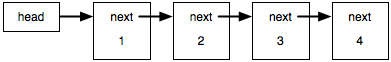
\includegraphics[scale=0.5]{proc-list-next.png} 
\vspace{1zh}
\end{center}
このリストを表現した二分探索木を1つ作り、節と枝(矢印)を用いて図示し なさい。ただし、木はバランスをしていなくても良いものとする。
注意: 正しい二分探索木は、複数存在する。
\end{screen}
\end{document}

